%%%%%%%%%%%%%%%%%%%%%%%%%%%%%%%%%%%%%%%%%
%
% 
%
%%%%%%%%%%%%%%%%%%%%%%%%%%%%%%%%%%%%%%%%%

%----------------------------------------------------------------------------------------
%	PACKAGES AND OTHER DOCUMENT CONFIGURATIONS
%----------------------------------------------------------------------------------------

\documentclass[paper=a4, fontsize=12pt]{scrartcl} % A4 paper and 11pt font size
\usepackage[]{algorithm2e} % Used for loading the algorithm package

%=-----------------------for diagram ---------
\usepackage{graphicx}



\usepackage{listings} % Required for inserting code snippets
\usepackage[usenames,dvipsnames]{color} % Required for specifying custom colors and referring to colors by name
\definecolor{DarkGreen}{rgb}{0.0,0.4,0.0} % Comment color
\definecolor{white}{RGB}{255,251,204} % Code highlight color

\lstdefinestyle{Style1}{ % Define a style for your code snippet, multiple definitions can be made if, for example, you wish to insert multiple code snippets using different programming languages into one document
language=Java, % Detects keywords, comments, strings, functions, etc for the language specified
backgroundcolor=\color{white}, % Set the background color for the snippet - useful for highlighting
basicstyle=\footnotesize\ttfamily, % The default font size and style of the code
breakatwhitespace=false, % If true, only allows line breaks at white space
breaklines=true, % Automatic line breaking (prevents code from protruding outside the box)
captionpos=b, % Sets the caption position: b for bottom; t for top
commentstyle=\usefont{T1}{pcr}{m}{sl}\color{DarkGreen}, % Style of comments within the code - dark green courier font
deletekeywords={}, % If you want to delete any keywords from the current language separate them by commas
%escapeinside={\%}, % This allows you to escape to LaTeX using the character in the bracket
firstnumber=1, % Line numbers begin at line 1
frame=single, % Frame around the code box, value can be: none, leftline, topline, bottomline, lines, single, shadowbox
frameround=tttt, % Rounds the corners of the frame for the top left, top right, bottom left and bottom right positions
keywordstyle=\color{Blue}\bf, % Functions are bold and blue
morekeywords={auto}, % Add any functions not included by default here separated by commas
numbers=left, % Location of line numbers, can take the values of: none, left, right
numbersep=10pt, % Distance of line numbers from the code box
numberstyle=\tiny\color{Gray}, % Style used for line numbers
rulecolor=\color{black}, % Frame border color
showstringspaces=false, % Don't put marks in string spaces
showtabs=false, % Display tabs in the code as lines
stepnumber=5, % The step distance between line numbers, i.e. how often will lines be numbered
stringstyle=\color{Purple}, % Strings are purple
tabsize=2, % Number of spaces per tab in the code
}

% Create a command to cleanly insert a snippet with the style above anywhere in the document
\newcommand{\insertcode}[2]{\begin{itemize}\item[]\lstinputlisting[caption=#2,label=#1,style=Style1]{#1}\end{itemize}} % The first argument is the script location/filename and the second is a caption for the listing



\usepackage[a4paper,pdftex]{geometry}	% Use A4 paper margins
\usepackage[english]{babel}
\usepackage{xcolor} % Required for specifying custom colors
\usepackage{fix-cm} % Allows increasing the font size of specific fonts beyond LaTeX default specifications

\setlength{\oddsidemargin}{0mm} % Adjust margins to center the colored title box
\setlength{\evensidemargin}{0mm} % Margins on even pages - only necessary if adding more content to this template

\newcommand{\HRule}[1]{\hfill \rule{0.2\linewidth}{#1}} % Horizontal rule at the bottom of the page, adjust width here

\definecolor{grey}{rgb}{0.9,0.9,0.9} % Color of the box surrounding the title - these values can be changed to give the box a different color	


%\usepackage{hyperref} %used for embedding url
\usepackage[T1]{fontenc} % Use 8-bit encoding that has 256 glyphs
\usepackage{fourier} % Use the Adobe Utopia font for the document - comment this line to return to the LaTeX default
\usepackage[english]{babel} % English language/hyphenation
\usepackage{amsmath,amsfonts,amsthm} % Math packages

\usepackage{lipsum} % Used for inserting dummy 'Lorem ipsum' text into the template

\usepackage{sectsty} % Allows customizing section commands
\allsectionsfont{\centering \normalfont\scshape} % Make all sections centered, the default font and small caps

\usepackage{fancyhdr} % Custom headers and footers
\pagestyle{fancyplain} % Makes all pages in the document conform to the custom headers and footers
\fancyhead{} % No page header - if you want one, create it in the same way as the footers below
\fancyfoot[L]{} % Empty left footer
\fancyfoot[C]{} % Empty center footer
\fancyfoot[R]{\thepage} % Page numbering for right footer
\renewcommand{\headrulewidth}{0pt} % Remove header underlines
\renewcommand{\footrulewidth}{0pt} % Remove footer underlines
\setlength{\headheight}{13.6pt} % Customize the height of the header

\numberwithin{equation}{section} % Number equations within sections (i.e. 1.1, 1.2, 2.1, 2.2 instead of 1, 2, 3, 4)
\numberwithin{figure}{section} % Number figures within sections (i.e. 1.1, 1.2, 2.1, 2.2 instead of 1, 2, 3, 4)
\numberwithin{table}{section} % Number tables within sections (i.e. 1.1, 1.2, 2.1, 2.2 instead of 1, 2, 3, 4)

\makeatletter
\newenvironment{chapquote}[2][2em]
  {\setlength{\@tempdima}{#1}%
   \def\chapquote@author{#2}%
   \parshape 1 \@tempdima \dimexpr\textwidth-2\@tempdima\relax%
   \itshape}
  {\par\normalfont\hfill--\ \chapquote@author\hspace*{\@tempdima}\par\bigskip}
\makeatother



\setlength\parindent{0pt} % Removes all indentation from paragraphs - comment this line for an assignment with lots of text

%----------------------------------------------------------------------------------------
%	TITLE SECTION
%----------------------------------------------------------------------------------------

\newcommand{\horrule}[1]{\rule{\linewidth}{#1}} % Create horizontal rule command with 1 argument of height

\title{	
\normalfont \normalsize 
\textsc{Indian Institute of Technology, Kanpur, CSE} \\ [25pt] % Your university, school and/or department name(s)
\horrule{0.5pt} \\[0.4cm] % Thin top horizontal rule
\huge CS698D, Assignment 1  \\ % The assignment title
\horrule{2pt} \\[0.5cm] % Thick bottom horizontal rule
}

\author{Harshit Maheshwari} % Your name

\date{\normalsize\today} % Today's date or a custom date

\begin{document}

%\maketitle
\thispagestyle{empty} % Remove page numbering on this page

%----------------------------------------------------------------------------------------
%	TITLE SECTION
%----------------------------------------------------------------------------------------

\colorbox{grey}{
	\parbox[t]{1.0\linewidth}{
		\begin{center}
		\fontsize{50pt}{80pt}\selectfont % The first argument for fontsize is the font size of the text and the second is the line spacing - you may need to play with these for your particular title
		\vspace*{0.7cm} % Space between the start of the title and the top of the grey box
		
		\hfill Java Extension:\\
		\hfill Automatic \\
		\hfill Type Inference\\
%		\hfill Clonable Interface\par
		\vspace{0.5cm}
		\end{center}				
		\raggedleft
		\fontsize{25pt}{12pt}\selectfont
		CS698Y Project, 2013-14 II
		\vspace*{0.7cm} % Space between the end of the title and the bottom of the grey box
		
	}
}

%----------------------------------------------------------------------------------------

\vfill % Space between the title box and author information

%----------------------------------------------------------------------------------------
%	AUTHOR NAME AND INFORMATION SECTION
%----------------------------------------------------------------------------------------

{\centering \large 
\hfill Abhimanyu Jaju \   \{\texttt{10327009, abhijaju@iitk.ac.in}\}\\
\hfill Harshit Maheshwari\ \{\texttt{10327290, harshitm@iitk.ac.in}\}\\
\hfill Vinit Kataria\ \{ \texttt{10327807, vinitk@iitk.ac.in}\}\\
\vspace{0.5cm}

\hfill Indian Institute of Technology, Kanpur \\
\hfill Computer Science and Engineering\\
%\hfill \texttt{harshitm@iitk.ac.in} \\



\HRule{1pt}} % Horizontal line, thickness changed here

%----------------------------------------------------------------------------------------

\clearpage % Whitespace to the end of the page

\tableofcontents
\newpage
\section{Abstract}
In Java, the type of a variable must be explicitly specified in order to use it. However, with our knowledge of type-inference and type-unification, usually we can deduce the types of variables as well as return types of functions (although it is not always possible to deduce the type). For this purpose we propose the use of auto keyword in Java. This would help developers to focus on the logic rather than on things which the compiler can itself deduce. The feature of auto keyword for type-deduction of variables has already been included in the latest C++11 standard. Further, in the proposed C++14 standard, automatic deduction of function-return-type has been included. 

\section{Keywords}
Java language features, auto, function type deduction, variable type deduction
%\section{Shallow Cloning vs Deep Cloning\label{shallowDeep}\cite{noAuthor1, Joe}}
The `object` class clone method by default returns shallow copy of the object. In order to create deep copy we need to override the `clone` method of the parent class.



\subsection{Shallow Cloning \label{shallow}}
As mentioned in Section \ref{introduction} `clone` method of `Object` class returns a shallow copy.
\insertcode{"Scripts/shallow2.java"}{Shallow Cloning\label{code:shallowCode}}
\insertcode{"Scripts/shallow2.output"}{Shallow Cloning Output\label{output:shallowCodeOutput}}


 As we can see from code \nameref{code:shallowCode} and the output \nameref{output:shallowCodeOutput} if the members of child class consists of 
\begin{itemize}
	\item \textbf{Primitive/Immutable data types}\\
	New copies are created. The value of primitive type `i` is copied in `cClone`.
	\item \textbf{User Defined classes}\\
	Only references are copied. Only the reference of field `StringBuffer b` is copied in clone `dClone`. 
\end{itemize}
The desired behaviour was to have different values in \textit{d.b} and \textit{dClone.b}. 
\subsection{Deep Cloning}
For deep cloning, we must satisfy following:\
\begin{itemize}
	\item All the members of the class  should implement Cloneable interface and should override Object's clone() method.
	\item If a member method does not follow the above rule, we must create a new instance of the member class and copy all the attributes to the new object(ensuring deep copying).
\end{itemize}

In order to implement the desired behaviour we need to modify the clone method of the child class as shown in Code \nameref{code:deepCode}
\insertcode{"Scripts/deep.java"}{`Deep Cloning`\label{code:deepCode}}
\insertcode{"Scripts/deep.output"}{`Deep Cloning Output` \label{output:deepCodeOutput}}

\section{State of Art}
Currently, Java supports no such feature. In Java, the  type of the variable and the return type of functions have to be explicitly mentioned at the time of variable/function declaration. However, the C++ language specifications have supports leaving the type deduction up to the compiler whenever possible in certain situations. The C++11 standard supports the keyword \textbf{auto} for variables which allows automatic type deduction for variables at compile time. Hence, at the time of variable declaration, the compiler deduces the type of the variable by looking at the value being assigned to it. Further, the new C++14 standard extends the usage of the keyword auto to function (as well as for lambda function) return-type-deduction. On similar lines, C\# standard currently supports the var keyword for automatic type deduction of variables. But, a necessity in both of the implementations is that the variable has to be initialized at the time of declaration. Another necessity is that if the function return type deduction has to be done by the compiler, then the function definition needs to accompany the function declaration.
\section{History and Usefulness of auto\cite{cppreference}}
The auto specifier was only allowed for variables declared at block scope or in function parameter lists. It indicated automatic storage duration, which is the default for these kinds of declarations. The meaning of this keyword was changed in C++11.\
\subsection{History}


\begin{chapquote}{Bjarne Stroustrup , \textit{C++11 - the new ISO C++ standard \cite{cppreference}}}

``The auto feature has the distinction to be the earliest to be suggested and implemented: I had it working in my Cfront implementation in early 1984, but was forced to take it out because of C compatibility problems. Those compatibility problems disappeared when C++98 and C99 accepted the removal of "implicit int"; that is, both languages require every variable and function to be defined with an explicit type. The old meaning of auto ("this is a local variable") is now illegal. Several committee members trawled through millions of lines of code finding only a handful of uses -- and most of those were in test suites or appeared to be bugs.\\
Being primarily a facility to simplify notation in code, auto does not affect the standard library specification.''
\end{chapquote}



\subsection{Usefulness}
Some powerful use of \textbf{auto} are described below:
\begin{itemize}
\item  \textbf{auto} can be used for iterating through object lists.
\insertcode{"Scripts/iterator.c"}{auto as iterator}
\item The use of auto to deduce the type of a variable from its initializer is obviously most useful when that type is either hard to know exactly or hard to write.
\insertcode{"Scripts/library.c"}{Type is hard to type/know \label{cyclicdependency3}}
\end{itemize}

%\section{Scope of Work and Expected Output}
\begin{itemize}
\item We propose to build a mini-compiler (toy implementation) which will support the basic functionalities of Java language with the above proposed functionality.
\item Making policies for handling the type-deduction for return type in functions when inheritance has to be taken care of while object type deduction.
\item Policies for unification of different types in return statements.
\item In some cases, types cannot be deduced in compile time for example
\insertcode{"Scripts/code4.java"}{}
In this case ‘a’ could be Dog or Cat and this depends on ‘b’. Such cases have to 
be carefully studied and need to be reported appropriately with 
warning/errors.
\end{itemize}
%\section{Proposed plan of work and techniques}
We plan to study the corresponding features existing in contemporary languages as mentioned above. 
For implementation purpose we plan to use one of the possible two approaches: 
\begin{itemize}
\item Study and extend some of the existing open source compilers specifically developed for studying compiler design like: Jastadd, Polyglot. 
\item  Develop a mini java compiler from scratch with the above proposed functionalities. 
\end{itemize}
The role of team members would be decided as we proceed with the project.
%\section{Outcome of the Project}
\begin{itemize}
\item Understanding of similar features that have been implemented in other languages, their method of implementation and the reasons behind introducing the new feature. 
\item Analyse in-depth the merits and demerits of introducing the proposed functionality in Java language.
\end{itemize}
\section{C++11 Specifications}
The C++11 specification for the use of `auto` keyword list the rules as follows: 
\begin{itemize}
\item The `auto` keyword can be used as a simple type specifier. Examples: 
\insertcode{"Scripts/autosyntaxc.c"}{Example assignment using `auto`}
\item `auto` can be used to provide a effective way for the programmers to express his intentions in context of objects. Examples: 
\insertcode{"Scripts/autosyntaxcobject.c"}{Reference type assignments using `auto`}
\item In C more than one variable can be declared in a single assignment provided that individual type deductions don't leave conflicts. 
\insertcode{"Scripts/autosyntaxcmulti.c"}{Multi Variable Declaration}
\item `auto` can be used for direct initialization, for the purpose of type deduction. Example: 
\insertcode{"Scripts/autosyntaxcdirect.c"}{Multi Variable Declaration}
\end{itemize}
\section{C++14 Proposed Plan}
Some of the proposals for C++14 language specification with reference to `auto` are mentioned below. 
\begin{itemize}
\item Allowing non-defining function declarations with auto return type is not strictly necessary, but it is useful for coding styles that prefer to define member functions outside the class. Example:
\insertcode{"Scripts/redeclaration.c"}{Forward declaration}
\item Since C++ compilers are single parse, if the return type cannot be deduced from the first return statement then it gives error. 
\insertcode{"Scripts/autosyntaxcfunction.c"}{Function return type deduction}
\item Similarly, for templates, some examples: 
\insertcode{"Scripts/autosyntaxcfunction.c"}{Template forward declaration}
\item Type deduction for multiple returns in a function is also defined. Examples: 
\insertcode{"Scripts/multiplereturns.c"}{Multiple returns in a function}
\item Recursion is handled in the following manner:
\insertcode{"Scripts/recursivec.c"}{Type deduction in recursive functions}
\end{itemize}
\section{Proposed Rules}
\subsection{`auto` for variables}
These rules discuss `auto` type assignment w.r.t. variables. 
\insertcode{"Scripts/code5.java"}{Example assignment for variables}
\subsubsection{`auto` for primitive data types}
If auto is used for variables then for primitive types we propose the following type assignments based on the range of the value to be assigned: 
\begin{table}[h]
\centering
\caption{Range for `type` assignment}
\begin{tabular}{|p{2cm}|p{5cm}|p{5cm}|}
\hline
\textbf{Primitive Type} & \textbf{Lower Range}  & \textbf{Upper Range}\\
\hline
%byte 			& 	-128 				& 127\\
%short 			&   -32,768				&	32,767\\
int 			& 	-2,147,483,648		&	2,147,483,647\\
long			&	(-9,223,372,036,854,775,808 \ ... \ -2,147,483,649)	& (2,147,483,648 \ ... \ 9,223,372,036,854,775,807)\\
float			& 	1.4E-45				& 3.4028235E+38\\
double  		&	439E-324			& 1.7976931348623157E+308\\
boolean 		& true	& false\\
\hline
\end{tabular}
\end{table}
However, as per the language specifications if `l` is appended in the numeral literal it is considered as a long literal by default. Similarly, if `f` is appended in the decimal literal it is considered as a float literal by default. 
\subsubsection{`auto` for user defined objects}
Suppose we have the following Class arrangement as shown in Figure 8.1.

\begin{figure}
\centering
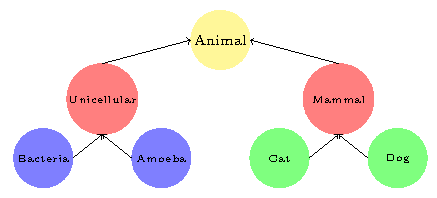
\includegraphics[width = 15cm]{diagram2.pdf}
\caption{Class Hierarchy Diagram\label{classhierarchy}}
\end{figure}

\insertcode{"Scripts/code6.java"}{Example assignment of user defined objects}

\subsection{`auto` for functions}
In the following code sample `x` would be assigned type `int` and `y` would be assigned type `Animal`. \\
\insertcode{"Scripts/code7.java"}{Basic function calling}

\subsubsection{Multiple return types for primitives}
\insertcode{"Scripts/code8.java"}{Multiple return types}
In case of conflicting return types of primitive data the function will return lowest common ancestor as shown in figure. Same rule will be followed for the wrapper class of these return types. 

\begin{figure}
\centering
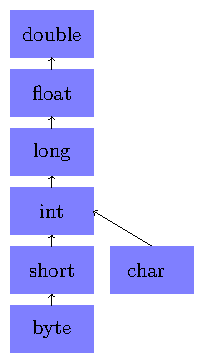
\includegraphics[width = 5cm]{diagram3.pdf}
\caption{Primitive data types coercision}
\end{figure}

\subsubsection{Multiple return types for classes}
\textbf{Parent $\leftrightarrow$ Child}\\
When the return type of a function is auto and it returns parent class as well as child class then after type resolution the parent class would be assigned as the return type of the function.

Based on the hierarchy of Figure 8.1 if we have the code as given in Listing 7 then the return type should be Animal.
\insertcode{"Scripts/code9.java"}{Multiple return types}
\textbf{Sibling $\leftrightarrow$ Sibling}\\
In case when the return type of the function is auto and it returns two sibling class in a class hierarchy then the return type of the function would be the lowest common ancestor in the inheritance hierarchy. 

Based on the hierarchy of Figure 8.1 if we have the code as given in Listing \ref{multireturntype1} then the return type should be Animal as it is the lowest common ancestor in the class hierarchy. 
\insertcode{"Scripts/code10.java"}{Multiple return types\label{multireturntype1}}
This is allowed because currently in Java the code given in Listing \ref{multireturntype2} is allowed. 
\insertcode{"Scripts/code11.java"}{Multiple return types\label{multireturntype2}}

\subsection{C/C++ Compiler}
In C++11 standards value assignment to `auto` variables cannot be deferred and the variable definition should be accompanied together with variable declaration.
Code given in Listing \ref{declareanddefine} is allowed but code given in Listing \ref{declareonly} gives error. 
\insertcode{"Scripts/code12.c"}{Immediate variable definition \label{declareanddefine}}
\insertcode{"Scripts/code13.c"}{Deferred variable definition \label{declareonly}}
C/C++ compilers are single parse compilers. Therefore, we need to give the function definition/declaration before actual function use. 
\subsubsection{Recursion}
The code given in Listing \ref{recurtionnotallowed1} and Listing \ref{recursionnotallowed2} should give error while the code given in Listing \ref{recursionallowed} is allowed. The reason is that we should know be able to deduce the  return type of functions in the first parse as C/C++ compilers are single parse.
\insertcode{"Scripts/code14.java"}{Not allowed\label{recurtionnotallowed1}}
\insertcode{"Scripts/code15.java"}{Not allowed\label{recursionnotallowed2}}
\insertcode{"Scripts/code16.java"}{Recursion allowed\label{recursionallowed}}

\subsection{Java Compiler}
We can allow the code given in Listing 15 in Java as Java compilers make multiple parse over the code. This is also the reason that in Java we can defer the function definition after function use because we can parse the code again to type check with the function definition. 
\insertcode{"Scripts/code17.java"}{Deferred variable definition}
In fact, in Java we can allow the use of `auto` keyword for function return type for cyclic dependencies as shown in Listing \ref{cyclicdependency1}. In Listing \ref{cyclicdependency1} the return type of all the functions will become `int`.
\insertcode{"Scripts/code18.java"}{Cyclic Dependency\label{cyclicdependency1}}
There is only one condition that it is actually possible to deduce the return type and there is not clash in return types. For instance the code given in Listing \ref{cyclicdependency2} will give compile time error as there is unresolved cyclic dependency of return types.
\insertcode{"Scripts/code19.java"}{Type deduction not possible\label{cyclicdependency2}}

However, the code given in Listing \ref{cyclicdependency3} is allowed and we can deduce the return type. 
\insertcode{"Scripts/code20.java"}{Cyclic dependencies\label{cyclicdependency3}}

\begin{figure}
\centering
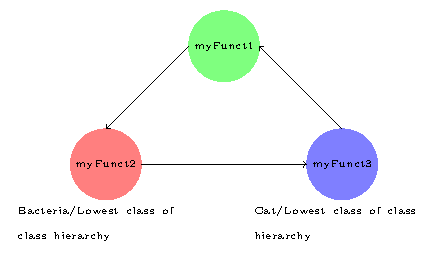
\includegraphics[width = 15cm]{diagram4.pdf}
\caption{Analysis of Listing 18}
\end{figure}
\section{Implementation}
As of now, we have implemented the following: 
\begin{itemize}
\item We have implemented a basic functionality providing Java compiler as the starting point for our project which supports compile time type deduction for variable declarations and return type of functions. We also generate assembly code for the same. 

\item We are doing type deductions only at compile time. 
\item \textbf{auto} can be used for type deductions of primitive as well as user defined types.
\insertcode{"Scripts/implemented.java"}{}

\item We have also generated assembly code for the same. 
\item We have also implemented type deductions for primitive function return type. 
\insertcode{"Scripts/implemented2.java"}{}

\item Automatic type coersion is also implemented for the same. 

\item Type deductions for \textbf{auto} functions with only one return statement which returns object is implemented. 
\insertcode{"Scripts/implemented3.java"}{}

\end{itemize}
The following is yet to be implemented: 
\begin{itemize}
\item Return type deduction for \textbf{auto} functions with multiple return statements that are returning different/same objects is yet to be implemented. 
\insertcode{"Scripts/implemented4.java"}{}

\item Return type inferencing for cyclic dependencies in functions is yet to implemented. 
\item Run time type deduction cases are yet to be implemented. 
\end{itemize}
\section{Acknowledgements}


\end{document}